\documentclass[review]{elsarticle}
\usepackage[margin=1in]{geometry}
\usepackage{lineno,hyperref}
\usepackage{amsmath}
\usepackage{xr-hyper}
\makeatletter
\newcommand*{\addFileDependency}[1]{% argument=file name and extension
  \typeout{(#1)}
  \@addtofilelist{#1}
  \IfFileExists{#1}{}{\typeout{No file #1.}}
}
\makeatother

\newcommand*{\myexternaldocument}[1]{%
    \externaldocument{#1}%
    \addFileDependency{#1.tex}%
    \addFileDependency{#1.aux}%
}
\myexternaldocument{supplement}

\newcommand{\etal}{\textit{et al.}}
\usepackage{xcolor}
\newcommand{\mike}[1]{\textcolor{red}{[Mike: #1]}}

\usepackage{endfloat}

\journal{American Journal of Human Genetics}


\bibliographystyle{elsarticle-num}
%%%%%%%%%%%%%%%%%%%%%%%

\begin{document}

\begin{frontmatter}

\title{Multi-omic strategies for transcriptome-wide prediction
    and association studies}

%% Group authors per affiliation:
\author{Arjun Bhattacharya\fnref{myfootnote}}
\fntext[myfootnote]{Department of Biostatistics,
University of North Carolina at Chapel Hill}

\author{Michael I. Love\fnref{myfootnote,myfootnote2}\corref{mycorrespondingauthor}}
\fntext[myfootnote2]{Department of Genetics,
University of North Carolina at Chapel Hill}

\cortext[mycorrespondingauthor]{Corresponding author}
\ead{milove@email.unc.edu}

\begin{abstract}
Traditional predictive models for transcriptome-wide association
studies (TWAS) consider only single nucleotide polymorphisms (SNPs)
local to genes of interest and perform parameter shrinkage
with a regularization process. These approaches ignore the effect of
distal-SNPs or possible effects underlying the SNP-gene
association. Here, we outline multi-omic strategies for transcriptome
imputation from germline genetics for testing gene-trait associations
by prioritizing distal-SNPs to the gene of interest. In one extension,
we identify mediating biomarkers (CpG sites, microRNAs, and
transcription factors) highly associated with gene expression and
train predictive models for these mediators using their local
SNPs. Imputed values for mediators are then incorporated into the
final model as fixed effects with local SNPs to the
gene included as regularized effects. In the second extension, we
assess distal-eSNPs (SNPs in eQTLs) 
for their mediation effect through mediators local
to these distal-eSNPs. Highly mediated distal-eSNPs are then included
in the eventual transcriptomic prediction model. We show considerable gains in percent variance explained of gene
expression and TWAS power to detect gene-trait associations
using simulation analysis and real data
applications with TCGA breast cancer data and in ROS/MAP brain tissue
data.  This
integrative approach to transcriptome-wide imputation and association
studies aids in understanding the complex interactions underlying
genetic regulation within a tissue and identifying important risk
genes for various traits and disorders.
\end{abstract}

\begin{keyword}
TWAS\sep GWAS \sep eQTL \sep mediation analysis
\end{keyword}


\end{frontmatter}

\section{Introduction}
Genomic methods that borrow information
from multiple data sources, or ``omics'' assays, offer advantages in
interpretability, statistical efficiency, and opportunities
to understand the flow of information in disease regulation
\cite{Hasin2017,Pinu2019}.
Transcriptome-wide association studies (TWAS)
aggregate genetic information
into functionally-relevant testing units that map
to genes and their expression in a relevant tissue.
This gene-based approach combines the effects
of many regulatory variants into 
a single testing unit that increases
study power and more interpretable trait-associated
genomic loci \cite{Gamazon2015,Gusev2016}. However,
traditional TWAS methods like PrediXcan and FUSION
focus on local genetic regulation of
transcription. These
methods ignore significant
portions of heritable
expression that can be attributed
to distal genetic variants
which may indicate complex
mechanisms that contribute
to gene regulation.

Recent work in transcriptional regulation has
estimated that distal genetic variants can account
for up to 70\% of the variance in gene expression 
\cite{Brynedal2017, Liu2019}. This result
accords with Boyle \etal{}'s omnigenic model,
proposing that regulatory networks are so
interconnected that a majority of genetic variants in
the genome, local or distal, have indirect effects on transcription of
any particular gene
\cite{Boyle2017, Liu2019}. Many groups have leveraged
this model to identify distal expression quantitative
trait loci (eQTLs) by testing
the effect of a distal-eSNP on an eGene
mediated through
a set of genes local to the SNP,
concluding that many distal-eQTLs are often
eQTLs for many local genes
\cite{Brown2013IntegrativeEQTLs,He2013Sherlock:GWAS,Pierce2014,Yang2017,Pierce2018Co-occurringMechanisms,Shan2019}.
It has been shown previously that
distal-eQTLs found in regulatory hotspots
are generally cell-type specific \cite{Brown2013IntegrativeEQTLs,Pierce2018Co-occurringMechanisms,vanderWijst2019Single-cellDisease}.
Deep learning methods have employed similar logic
to link GWAS-identified variants to nearby regulatory mechanisms
for functional hypothesis generation \cite{Arloth2020DeepWAS:Learning}.
Furthermore, Zhang \etal{}'s recent EpiXcan method demonstrates
that incorporating epigenetic information into transcriptomic
prediction models generally improves predictive performance
and power in detecting gene-trait associations in TWAS \cite{Zhang2019}.

Here, we outline two extensions to TWAS,
borrowing information from other omics assays to enrich or prioritize
mediator relationships of eQTLs in expression models.
Using simulations and 
data from the The Cancer Genome
Atlas (TCGA) \cite{McLendon2008} 
and the Religious Orders Study and 
the Rush Memory and Aging Project (ROS/MAP) \cite{DeJager2018},
we show improvements in 
transcriptomic prediction
and power to detect
gene-trait associations.
These \textbf{M}ulti-\textbf{O}mic \textbf{S}trategies for \textbf{T}ranscriptome-\textbf{W}ide
\textbf{A}ssociation \textbf{S}tudies are curated in the R package MOSTWAS,
available freely at \url{www.github.com/bhattacharya-a-bt/MOSTWAS}.


\section{Material and Methods}
We first outline the two methods
proposed in this work, (1) mediator-enriched transcriptome-wide
prediction (MeTWAS) and (2) distal-eQTL 
prioritization via mediation analysis (DePMA). 
MeTWAS and DePMA are combined
in the MOSTWAS R package,
available freely at \url{https://bhattacharya-a-bt.github.io/MOSTWAS}.

\subsection{Mediator-enriched TWAS (MeTWAS)}

\subsubsection{Transcriptomic prediction using MeTWAS}

Here, we present mediator-enriched TWAS, or MeTWAS
one of the two tools presented in the MOSTWAS R package.
Across $n$ samples, consider the vector $Y_G$,
the expression of a gene $G$ 
of interest, the matrix $\mathbf{X}_G$ 
of local SNPs dosages
in a user-defined window around gene $G$ (default to 0.5 Megabases), 
and $m_G$ mediating biomarkers that
we estimate to be significantly associated
with the expression of gene $G$ via a
relevant one-way test of association. These
mediating biomarkers can be DNA methylation sites,
microRNAs, transcription factors, or any
molecular profile that may be genetically
heritable and affect transcription. Accordingly,
let the matrix $\mathbf{X}_{M_j}$ be the 
local-genotype dosages in a 500 kilobase
window around mediator $j,~1 \leq j \leq m_G$. Furthermore,
let $M_j$ be the intensity of mediator $j$ 
(methylation $M$-value if $j$ is a CpG site,
expression if $j$ is a miRNA or a gene, etc).
Prior to any modelling, we scale $Y_G$ and all 
$M_j,~1 \leq j \leq m_G$ to zero mean and
unit variance. We also residualize
$M_j,~1 \leq j \leq m_G$ and $Y_G$ 
with the covariate matrix $\mathbf{X}_C$
to account for population stratification using
principal components of the global genotype matrix
and relevant clinical covariates to obtain
$\tilde{M}_j,~1 \leq j \leq m_G$ and $\tilde{Y}_G$.

Transcriptome prediction in MeTWAS draws from
two-step regression, as summarized in \textbf{Figure \ref{fig:ch4_fig1}}.
First, in the training set
for a given training-test split,
for $1 \leq j \leq m_G$, we model the residualized 
intensity $\tilde{M}_j$ of training-set specific 
mediator $j$ with
the following additive model:

\begin{equation}
	\tilde{M}_j = \mathbf{X}_{M_j,train}w_j +
	\varepsilon_m,
\end{equation}

\noindent where $w_j$ is the effect-sizes of
the SNPs in $\mathbf{X}_{M_j,train}$ on $\tilde{M}_j$
in the training set.
As in traditional transcriptomic
imputation models \cite{Gamazon2015,Gusev2016},
we find $\hat{w}_j$ using
one of the two following methods
with the largest predicted adjusted $R^2$: 
(1) elastic net regression with mixing parameter $\alpha = 0.5$
and $\lambda$ tuned over 5-fold cross validation
using glmnet \cite{Friedman2010}, or
(2) linear mixed modelling assuming random effects
for $\mathbf{X}_{M_j}$ using rrBLUP \cite{Endelman2011}.
Only significantly heritable (default $P < 0.05$
for the likelihood ratio test) \cite{Yang2015} and
well-cross validated (default $R^2 \geq 0.01$)
expression models
are considered.

For all $j$, using these optimized predictive
models for $M_j$ as denoted
by $\hat{w}_{M_j}$, 
we estimate the genetically regulated
intensity (GRIn) of the mediator $m_j$, denoted
GRIn$_{m_j}$, in the test set. Denote
$\mathbf{\hat{M}}$ as the $n \times m$
matrix of estimated GRIn, such that
the $j$th column of $\mathbf{\hat{M}}_j$ is
GRIn$_{m_j}$ across all $n$ samples. 

Next, we consider
the following additive model for
the residualized expression of gene $G$:


\begin{equation}\label{2sls}
\begin{split}
\tilde{Y}_G & = \mathbf{M}\beta_{\mathbf{M}} + \varepsilon_{Y_{G_1}}, \\
\tilde{Y}_G - \mathbf{M}\hat{\beta}_{\mathbf{M}} & = \mathbf{X}_G\beta_{M} + \varepsilon_{Y_{G_2}}.
\end{split}
\end{equation}

\noindent where $\beta_M$ is the fixed effect-sizes
of GRIn$_{m_j}$ on $\tilde{Y}_G$, $\hat{\mathbf{M}}$
is the matrix of estimated GRIn for
all $m_j$ mediators, $\mathbf{X}_G$
are the local-SNPs to gene $G$, and $w_G$
are the ``random'' or regularized 
effect sizes of the local-SNPs.
We first estimate $\hat{\beta}_M$ by
traditional ordinary least squares, where
$\hat{\beta}_M = \left(\mathbf{\hat{M}}'\mathbf{\hat{M}}\right)^{-1}\mathbf{\hat{M}}'E_g$.
Next, using one of the methods outlined above
when estimating $\hat{w}_{M_j}$, we
can estimate the effect sizes $\hat{w}_G$ 
of the local-SNPs on $\tilde{Y}_G$, residualized
with $\hat{\mathbf{M}}$, using
either elastic net or linear mixed models \cite{Friedman2010,Endelman2011}. 

\subsubsection{Transcriptomic imputation with MeTWAS}
In an external GWAS panel, if individual SNPs are 
available, we construct the mediator-enriched genetically regulated
expression (MeGReX) of gene $G$
directly using $\hat{w}_G$ and $(\hat{w}_j,\hat{\beta}_j),~1 \leq j \leq m_G$:

$$MeGReX_G = \sum_{j =two 1}^{m_G}{\mathbf{X}_{M_j,GWAS}\hat{w}_{M_j}\hat{\beta}_{M,j}} + 
\mathbf{X}_{G,GWAS}\hat{w}_G,$$

\noindent where $\mathbf{X}_{M_j,GWAS}$ and $\mathbf{X}_{G,GWAS}$ 
are the SNPs in the GWAS
panel local to mediator $j$ and gene $G$, respectively.
$MeGREX_G$ can be used in downstream tests of association. 


\subsection{Distal-eQTL prioritization via mediation analysis (DePMA)}

\subsubsection{Transcriptomic prediction using DePMA}

Expression prediction in DePMA hinges on
assessing distal-eSNPs for inclusion in the design matrix
via mediation analysis, adopting
methods from previous studies \cite{Pierce2014,Shan2019,Yang2017}. 
We first split data for
gene expression, SNP dosages, and any potential mediators
into $k$ training-testing splits. Based on the 
minor allele frequencies of SNPs and sample size,
we recommend a low number of splits (i.e. $k \leq 5$).

In the training set, we identify mediation test triplets
that consist of (1) a gene of interest $G$
with expression $Y_G$ (scaled to zero mean
and unit variance), (2)
a distal-eSNP $s$ in association
with $G$ at a user-defined $P$-value
threshold (default of $P = 10^{-6}$)
with dosages $X_s$, and (3)
a set of $m$ biomarkers local 
to $s$ that are associated
with $s$ at a user-defined $P$-value threshold
(default of FDR-adjusted $P = 0.05$)
with intensities in the $m$ columns of 
$\mathbf{M}$. The columns of $\mathbf{M}$
are scaled to zero mean and unit variance.
Consider the following
mediation model:

\begin{equation}\label{mediation}
\begin{split}
Y_G & = X_s\beta_s + \mathbf{M}\beta_{\mathbf{M}} + \mathbf{X}_C\beta_{C} + \varepsilon_{Y_G} \\
M_j & = X_s\alpha_{M_j} + \mathbf{X}_C\alpha_{C,j} + \varepsilon_{M_j}, \quad 1 \leq j \leq m.
\end{split}
\end{equation}

Here, we have $\beta_{\mathbf{M}}$ as the
effects of the $M$ mediators local to $s$ on $Y_G$ adjusting
for the effects from $s$ and the covariates $\mathbf{X}_C$, and 
$\alpha_{\mathbf{M}} = (\alpha_{M_1},\ldots,\alpha_{M_m})'$
as the effects of $s$ on mediators $M_j$, for $1 \leq j \leq m$.
We assume that $\varepsilon_{Y_G} \sim N(0,\sigma^2)$ and 
$\varepsilon_{\mathbf{M}} \sim \mathbf{N}_m\left(0,\mathbf{\Sigma}_M\right)$,
where $\mathbf{\Sigma}_M$ may have non-zero off-diagonal
elements that
represent non-zero covariance between mediator
intensities. 
Further, we assume that $\varepsilon_{Y_G}$ and
$\varepsilon_{\mathbf{M}}$ are independent.
We define the total mediation effect
(TME) 
\cite{Sobel1982AsymptoticModels} of SNP $s$
as 

$$TME = \alpha_{\mathbf{M}}^T\beta_{\mathbf{M}}.$$

\noindent We are interested in SNPs with large absolute TME, which
we assess with a two-sided test of $H_0:~TME = 0$.
We assess this hypothesis with a permutation test to obtain a
permutation $P$-value,
as more direct methods of computing standard errors
for the estimated TME are often biased \cite{Mackinnon2004,Shan2019},
We also provide an option to estimate
an asymptotic approximation to the
standard error of $TME$ 
and conduct a Wald-type test for
$H_0:~TME = 0$. This asymptotic option 
is significantly faster at
the cost of inflated false positives 
(see \textbf{Supplemental Materials}
and 
\textbf{Supplemental Figure \ref{fig:ch4_fig2}}).
Corresponding to the $t$ testing triplets identified, 
we obtain vectors of length $t$ of TMEs and $P$-values
for each distal-eSNP to $G$. We estimate
the $q$-value for each test to adjust
for multiple testing \cite{Storey2019b}.
For the predictive model, we select distal
SNPs with $TME \neq 0$ 
at a given $q$-value threshold ($q < 0.10$
as a default)
and include them with all local SNPs in
a design matrix. We then find estimated SNP
weights using either elastic net or weighted least
squared regression.

\subsubsection{Transcriptomic imputation with DePMA}
In an external GWAS panel, if individual SNPs are 
available, we construct the genetically regulated
expression (GReX) of gene $G$
directly using $\hat{w}_G$ and $\hat{w}_t$:

$$GReX_G = \mathbf{X}_{t,GWAS}\hat{w}_{t} + 
\mathbf{X}_{G,GWAS}\hat{w}_G,$$

\noindent where $\mathbf{X}_{t,GWAS}$ is the matrix of dosages of the
$t$ distal-SNPs and $\mathbf{X}_{G,GWAS}$ is the matrix of 
dosages of the local SNPs to gene $G$ in the external GWAS
panel. $GREX_G$ can be used in downstream tests of association.
If individual SNPs are not available, the weighted
burden test can be employed using summary statistics with
permutation follow-up
test \cite{Gusev2016}.

\subsection{Tests of associations}


If individual SNPs are not available, then the weighted burden
$Z$-test proposed by Gusev \etal{} can be employed \cite{Gusev2016} 
using
summary statistics. Briefly, we compute

\begin{equation}\label{wbtest}
\begin{split}
\tilde{Z} & = \frac{\mathbf{W}Z}{(\mathbf{W}\Sigma_{s,s}\mathbf{W}^T)^{1/2}}.
\end{split}
\end{equation}

Here, $Z$ is the vector of $Z$-scores of SNP-trait
associations for SNPs used in estimating $\hat{w}_{M_j}$
and $\hat{w}_G$. The matrix $\mathbf{W}$ is defined as 
$\Sigma_{e,s}\Sigma_{s,s}^{-1}$, the product of
the covariance matrix between all SNPs
and the expression of gene $G$ and the covariance
matrix among all SNPs. These covariance matrices
are estimated from the eQTL reference panel used to estimate
$\hat{w}_{M_j}$
and $\hat{w}_G$.
and $\hat{w}_G$. The test statistic $\tilde{Z}$
can be compared to the standard Normal distribution
for inference.
We implement a permutation
test conditioning
on the GWAS effect sizes to assess
whether the same distribution
of $\hat{w}_G$ effect
sizes could yield a significant
association by chance \cite{Gusev2016}. 
We
permute $\hat{w}_G$ 1,000
times without replacement
and recompute the weighted
burden test statistic
to generate a permutation
null distribution for $\tilde{Z}$.
This permutation test
is only conducted for
overall associations
at a user-defined significance
level (default to FDR-adjusted $P < 0.05$). 

Lastly, we also 
implement a test to assess
the information added from distal-eSNPs
in the weighted burden test beyond
what we find from local SNPs.
This test is analogous to a group added-last test in regression
analysis, applied here to GWAS summary statistics.
Let $Z_l$ and 
$Z_d$  be the vector of $Z$-scores
from GWAS summary statistics
from
local and distal-SNPs identified
by a MOSTWAS model. 
The local
and distal-SNP effects
from the MOSTWAS model are represented
in $\mathbf{w}_l$ and 
$\mathbf{w}_d$.
Formally, we test
whether the weighted $Z$-score $\tilde{Z}_d \equiv \mathbf{w}_d^TZ_d$
from distal-SNPs is significantly
larger than 0 given the observed
weighted $Z$-score from local SNPs $\tilde{Z}_{l} \equiv \mathbf{w}_l^TZ_l$,
drawing from the assumption that
$(\tilde{Z}_l,\tilde{Z}_d)$
follow a bivariate Normal distribution. Namely, we
conduct a two-sided
Wald-type test for the null
hypothesis:

$$H_0: \mathbf{w}_d^T\mathbf{Z}_d | \mathbf{w}_l^T\mathbf{Z}_l = \tilde{Z}_{l,\text{obs}} = 0.$$

\noindent Under the null hypothesis,
we can derive that 
$\tilde{Z}_d|\tilde{Z}_l = \tilde{Z}_{l,\text{obs}}$
is normally distributed
with mean and variance
determined from the observed
local $\tilde{Z}_l$-score,
the SNP-effect size
vectors $\mathbf{w}_l$
and $\mathbf{w}_d$,
and components of the linkage
disequilibrium as estimated
from the reference panel \cite{Pasaniuc2014FastEnrichment}.
Full details and derivation
for this added-last test
are given in \textbf{Supplemental
Methods}.

\subsection{Simulation framework}

We first conducted simulations to assess
the predictive capability
and power to detect
gene-trait associations
under various phenotype heritability ($h^2_p$),
local heritability of expression ($h^2_{e,l}$),
distal heritability of expression ($h^2_{e,d}$),
and proportion of causal local ($p_{c,l}$)
and distal ($p_{c,e}$) SNPs
for MeTWAS and DePMA.
We considered two scenarios for each
combination of $(h^2_p, h^2_{e,l}, h^2_{e,d}, p_{c,l},
p_{c,e})$: (1) the leveraged association
between the distal-SNP and gene of interest
exists in both the reference
and imputation panel, and (2) the leveraged association 
between distal-SNP and gene of interest
exists in the reference panel but is null
in the imputation panel.

Using TCGA data, we 
extracted 2,592 SNPs local to
the gene \emph{ESR1} 
on Chromosome 6 and 1,431 SNPs
local to the gene \emph{FOXA1}.
We generated (1) a reference panel with sample
size 400 with
simulated SNPs, expressions,
and one mediator
and (2) a GWAS panel of
1,500 samples with simulated SNPs
and phenotypes using the following data
generating process, modified
from Mancuso \etal{}'s framework
\cite{Mancuso2019ProbabilisticStudies}:

We estimated the linkage disequilibrium $LD$
matrix of the SNPs $X_G$ with $n$
samples and $p$ SNPs, as follows
with regularization to ensure $LD$ is positive semi-definite:

$$LD = \frac{1}{n}X_G^TX_G + \frac{1}{10}I_p.$$ 

\noindent We computed the Cholesky decomposition of
$LD$ for faster sampling
\cite{Mancuso2019ProbabilisticStudies}.
We simulated SNPs for a 400-sample
reference panel $X_{g,ref}$ and 
1,500-sample GWAS panel $X_{g,GWAS}$.

We then simulated
effect sizes for $p_{c,l}$ of
the 2,592 local
SNPs $w_{g,l}$ 
from a standard Normal distribution.
We generated locally heritable
expression 

$$E_{g,l} = X_{G,ref}^Tw_{g,l} + \varepsilon_l,$$

\noindent with $\varepsilon_l \sim N(0,1-h^2_{e,l})$
and $w_{g,l}$ scaled to ensure the given $h^2_{e,l}$.
Similarly, we simulated effect sizes
for $p_{c,d}$ of the 1,431 distal-SNPs
$w_{g,d}$ and generated the distally heritable
intensity of the mediator $M_{g,d}$. We constructed
the distally heritable expression $E_{g,d}$
by scaling $M_{g,d}$ by $\beta \sim N(0,1)$ and adding random noise
that scales distal heritability to $h^2_{e,d}$.
We lastly formed the total expression $E_g = E_{g,l} + E_{g,d}$.

Next, we simulated the phenotype
in the GWAS panel using the GREx as
estimated from causal eQTLs to match
the variance explained due to genetics. We drew a
causal effect size from gene expression $\alpha \sim N(0,1)$.
We computed the unobserved gene expression
in the GWAS panel as

$$E_{g,GWAS}|X_{g,GWAS,local},X_{g,GWAS,distal} = X_{g,GWAS,local}^Tw_{g,l} + 
X_{g,GWAS,distal}^Tw_{g,d}\beta + \varepsilon_{GWAS}.$$

\noindent Here, we also considered a ``null'' case as well, where the
simulated
distal eQTLs do not contribute to the simulated phenotype in the GWAS panel 
(i.e. $w_{g,d} = 0$
for all distal-SNPs). GWAS summary statistics
were computed in this step for downstream weighted
burden testing.
We then fitted predictive models using MeTWAS, DePMA,
and local-only models (i.e. FUSION \cite{Gusev2016}),
computed the adjusted predictive $R^2$
in the reference panel, and tested
the gene-trait association in the GWAS panel
using a weighted burden test.
The association study power was defined
as the proportion of gene-trait association
tests with $P < 2.5 \times 10^{-6}$,
the Bonferroni-corrected significance threshold
for testing 20,000 independent genes.
With these simulated datasets,
we also assessed the power
of the distal added-last test
by computing the proportion
of significant distal associations
conditional on the local association
at FDR-adjusted $P < 0.05$.

\subsection{Data acquisition}

\subsubsection{Multi-omic data from TCGA-BRCA}

We retrieved genotype, RNA expression,
miRNA expression, and DNA methylation data
for breast cancer indications in The Cancer Genome Atlas (TCGA).
Birdseed genotype files of 914 subjects were downloaded
from the Genome Data Commons (GDC)
legacy (GRCh37/hg19) archive. Genotype
files were merged into a single binary PLINK
file format (BED/FAM/BIM) and imputed
using the October 2014 (v.3) release of the 1000 Genomes
Project dataset as a reference panel in
the standard two-stage imputation approach,
using SHAPEIT v2.87 for phasing and IMPUTE
v2.3.2 for imputation
\cite{OConnell2014,Delaneau2012,Howie2009}.
We excluded variants (1) with a minor
allele frequency of less that 1\% based on
genotype
dosage, (2) that deviated significantly from
Hardy-Weinberg equilibrium ($P < 10^{-8}$)
using appropriate functions in PLINK v1.90b3
\cite{Wigginton2005,Purcell2007}, and
(3) located on sex chromosomes.  
Final TCGA genotype data was coded as dosages,
with reference and alternative allele coding as in
dbSNP.

TCGA level-3 normalized RNA-seq expression data,
miRNA-seq expression data, and DNA methylation
data collected on Illumina Infinium HumanMethylation450 BeadChip were downloaded
from the Broad Institute's GDAC Firehose (2016/1/28
analysis archive) via FireBrowse \cite{Weinstein2013TheProject}. We intersected to the subset
of samples assayed for
genotype (4,564,962 variants), 
RNA-seq (15,568 genes), 
miRNA-seq (1,046 miRNAs),
and DNA methylation (485,578 CpG sites), 
resulting in a total
of 563 samples. We only considered
the autosome in our analyses.
We adjusted gene and miRNA expression
and DNA methylation by relevant
covariates (10 principal 
components of the genotype 
matrix, tumor stage at diagnosis,
and age).

\subsubsection{Multi-omic data from ROS/MAP}

We retrieved imputed genotype, RNA expression,
miRNA expression, and DNA methylation data
from The Religious Orders Study and Memory and Aging Project (ROS/MAP) Study
for samples derived from human pre-frontal cortex
\cite{A.Bennett2013OverviewStudy,A.Bennett2013OverviewProject,DeJager2012ADecline,DeJager2018DataResearch}.We excluded variants (1) with a minor
allele frequency of less that 1\% based on
genotype
dosage, (2) that deviated significantly from
Hardy-Weinberg equilibrium ($P < 10^{-8}$)
using appropriate functions in PLINK v1.90b3
\cite{Wigginton2005,Purcell2007}, and
(3) located on sex chromosomes. 
Final ROS/MAP genotype data was coded as dosages,
with reference and alternative allele coding as in
dbSNP. We intersected to the subset
of samples assayed for 
genotype (4,141,537 variants), 
RNA-seq (15,857 genes), 
miRNA-seq (247 miRNAs),
and DNA methylation (391,626 CpG sites), resulting in a total
of 370 samples. Again, we only considered
the autosome in our analyses.
We adjusted gene and miRNA expression
and DNA methylation by relevant
covariates (10 principal 
components of the genotype 
age at death, sex, and smoking status).

\subsubsection{Summary statistics
for downstream association studies}

We conducted TWAS association tests
using relevant GWAS summary statistics
for breast cancer-specific survival, risk of late-onset Alzheimer's disease, and
risk of major depressive disorder.
We downloaded
iCOGs GWAS summary statistics for
breast cancer-specific survival for
women of European ancestry \cite{Guo2015}.
All studies and 
funders as listed in Michailidou
\etal{} \cite{Michailidou2013,Michailidou2015} 
and in Guo \etal{} \cite{Guo2015} 
are acknowledged for their contributions.
Furthermore, we downloaded
GWAS summary statistics for risk of
late-onset Alzheimer's disease 
from the International Genomics
of Alzheimer's Project (IGAP)
\cite{Lambert2013Meta-analysisDisease}.
We also downloaded GWAS and genome-wide
association by proxy (GWAX) summary statistics
for risk of major depressive
disorder (MDD) from the Psychiatric Genomics
Consortium \cite{Wray2018Genome-wideDepression}
and the UK Biobank \cite{Liu2017Case-controlDisease}, respectively.
IGAP is a large two-stage study based on GWAS 
on individuals of European ancestry. 
In stage~1, IGAP used genotyped and 
imputed data on 7,055,881 single 
nucleotide polymorphisms (SNPs) to 
meta-analyze four previously-published
GWAS datasets consisting of 17,008
Alzheimer's disease cases and 
37,154 controls (The European 
Alzheimer's disease Initiative --
EADI the Alzheimer Disease Genetics 
Consortium -- ADGC The Cohorts for
Heart and Aging Research in Genomic 
Epidemiology consortium -- CHARGE The 
Genetic and Environmental Risk in AD 
consortium -- GERAD). In stage~2, 11,632
SNPs were genotyped and tested for 
association in an independent set of 
8,572 Alzheimer's disease cases and 
11,312 controls. Finally, a 
meta-analysis was performed combining results from stages 1 and 2.

\subsection{Model training
and association testing in
TCGA-BRCA and ROS/MAP}

Using both TCGA-BRCA and
ROS/MAP multiomic
data, we first identified
associations between
SNPs and mediators (transcription
factor genes, miRNAs, and
CpG methylation sites),
mediators and gene expression,
and SNPs and gene expression
using MatrixEQTL
\cite{Shabalin2012a}.
These QTL analyses were
adjusted for 10 principal
components of the genotype
matrix to account for 
population stratification,
along with other relevant
covariates (tumor stage and age
for TCGA-BRCA, age and sex and smoking status for ROS/MAP).
For MeTWAS modeling, we considered
the top 5 mediators associated
with the gene of interest, assessed
by the smallest FDR-adjusted $P < 0.05$.
For DePMA models, we considered
all distal-SNPs
associated with gene expression
at raw $P < 10^{-6}$
and any local mediators at
FDR-adjusted $P < 0.05$.
Local windows for all models
were set to 0.5 Mb. For association
testing, we consider
only genes with significant 
non-zero
estimated total
heritability by
GCTA-LDMS \cite{Yang2015}
and cross-validation
adjusted $R^2 > 0$
across 5 folds.
The MeTWAS or DePMA
model with larger cross-validation
$R^2$ was considered
as the final MOSTWAS model
for a given gene. All
other modeling options
in MeTWAS and DePMA
were set to the defaults
provided by the MOSTWAS package.

Using TCGA-BRCA models,
we conducted TWAS burden testing
\cite{Pasaniuc2014FastEnrichment,Gusev2016} in iCOGs
GWAS summary statistics
for breast cancer-specific
survival in a cohort
of women of European ancestry.
We subjected TWAS-identified loci
at Benjamini-Hochberg \cite{Benjamini1995} 
FDR-adjusted $P < 0.05$
to permutation testing,
and any loci that persisted
past permutation testing to
distal variation
added-last testing.

Using ROS/MAP models,
we first conducted 
TWAS burden testing
in GWAS summary statistics
for late-onset
Alzheimer's disease risk
from IGAP, prioritized
14 known risk loci identified
from literature 
\cite{Lambert2013Meta-analysisDisease,Reitz2014GeneticDisease,Sims2017RareDisease,Yuan2017TheDisease}.
We subjected TWAS-identified loci
at Benjamini-Hochberg \cite{Benjamini1995} 
FDR-adjusted $P < 0.05$
to permutation testing,
and any loci that persisted
past permutation testing to
distal variation
added-last testing.
We similarly conducted TWAS
for risk of major
depressive disorder (MDD)
using GWAS summary statistics
from PGC (excluding data
from 23andMe and the UK Biobank)
with the necessary follow-up
tests. For any TWAS-identified loci
that persisted
permutation in PGC,
we further conducted TWAS
in GWAX summary statistics 
for MDD risk in
the UK Biobank
\cite{Liu2017Case-controlDisease}
for replication.


\section{Results}
\subsection{Overview of MOSTWAS}

MOSTWAS incorporates two
methods to include distal-eQTLs
in transcriptomic prediction: mediator-enriched
TWAS (MeTWAS) and distal-eQTL prioritization
via mediation analysis (DePMA). 
As large proportions of total
heritable gene expression are explained
by distal-eQTLs local to regulatory
hotspots 
\cite{Liu2019,Pierce2014,Pierce2018Co-occurringMechanisms,Shan2019},
we used data-driven approaches
to either identify mediating
regulatory biomarkers (MeTWAS)
or distal-eQTLs mediated by 
local biomarkers (DePMA) to
increase predictive power and
power to detect gene-trait associations.
We assess in-sample predictive performance of MeTWAS and DePMA
via cross-validation over a user-defined $k$ folds
of training and test sets,
such that the expression model is estimated
in the training set and imputed into the test set
for cross-validation.
These
methods are summarized graphically
in \textbf{Figure \ref{fig:ch4_fig1}}.


\begin{figure}[!h]
	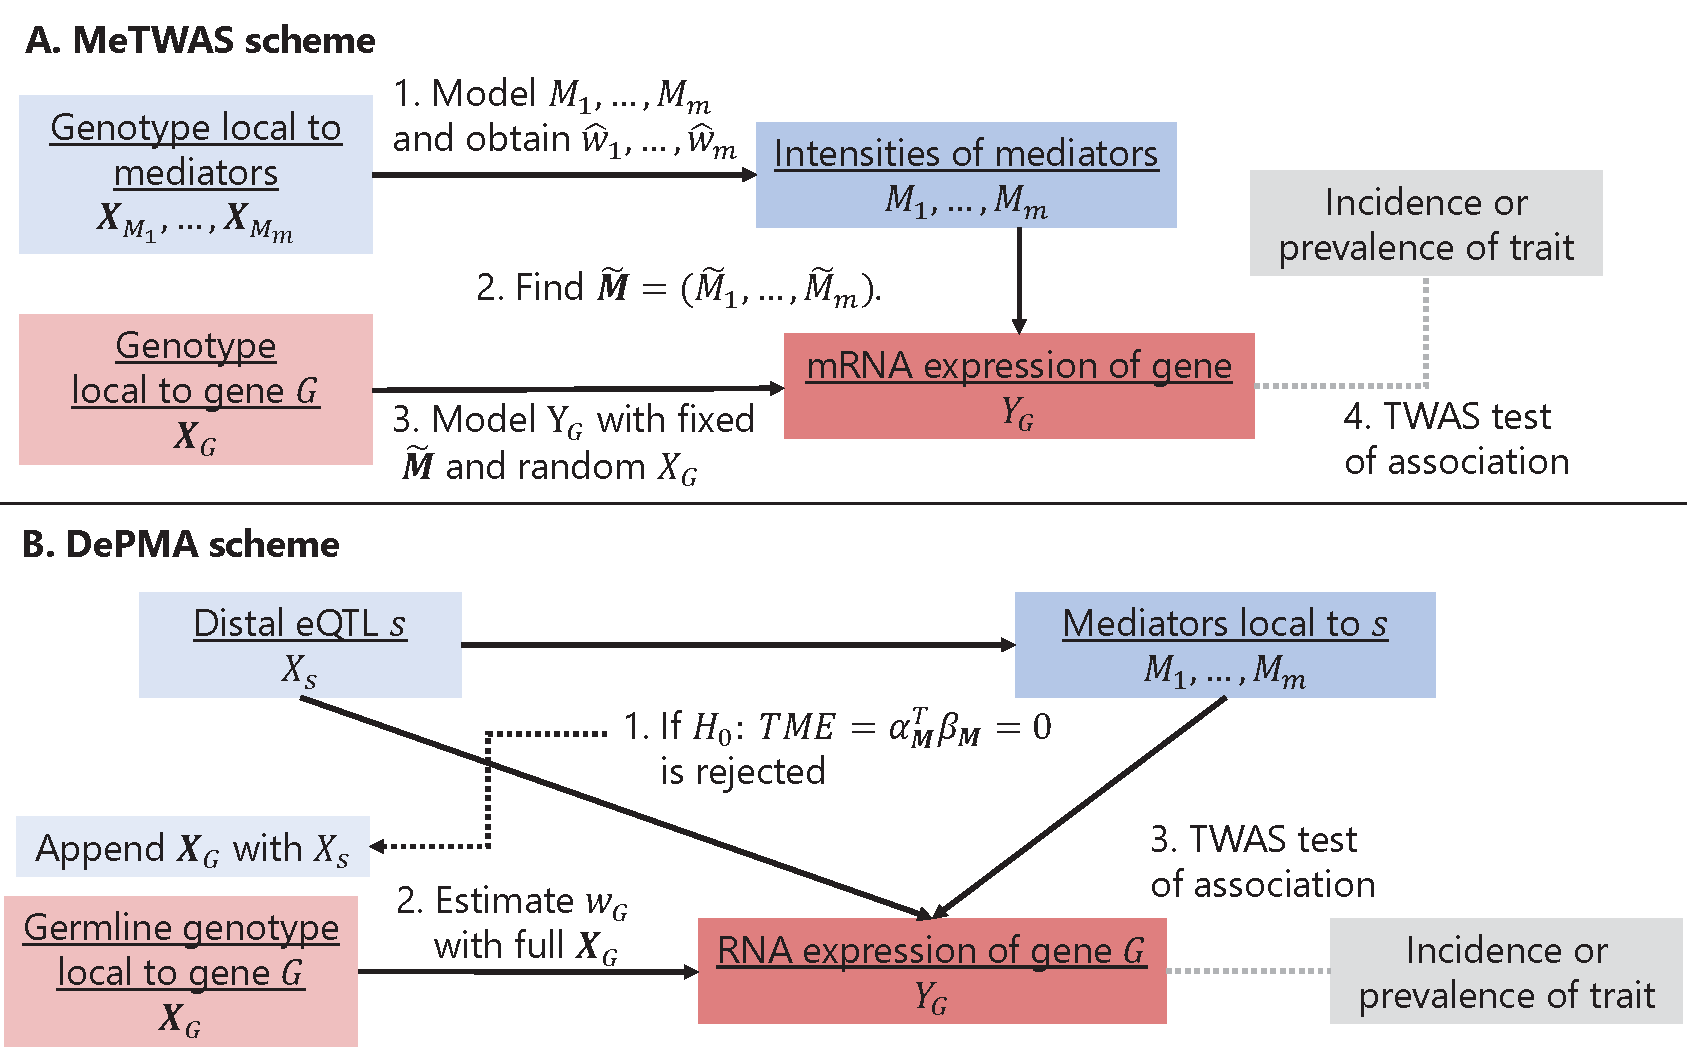
\includegraphics[width = \textwidth]{figures/ch4_fig1.pdf}
	\caption{\emph{Modeling schemes
	implemented in MOSTWAS.} (A) 
	Two-step least squares for mediator-enriched
	TWAS (MeTWAS). (B)
	Distal-eQTL prioritization by
	via mediation analysis (DePMA).}
	\label{fig:ch4_fig1}
\end{figure}

\begin{itemize}

\item MeTWAS first
identifies $m$ potential mediators
(e.g. CpG sites,
miRNAs, genes coding
for transcription
factors, etc) such
that the intensity (methylation, 
expression levels, etc) 
of these mediators are associated
with the mRNA expression of the gene of interest.
A model for the
genetically regulated intensities
(GRIn)
is estimated using
the local SNPs
to these mediators, and
the GRIn of these mediators
are imputed into the training
set.
The final gene expression model
is estimated by incorporating
the GRIn of the mediators
as fixed effects and 
the local SNPs 
to the gene as regularized
effects (see \textbf{Methods}
for more details).

\item DePMA
first identifies
testing triplets
of the gene of
interest, a distal
eSNP (SNP
in an eQTL) to the gene,
and any potential associated mediators local
to the eQTL. 
The total mediation effect (TME) 
of the eQTL on the gene 
through the set of mediators
is estimated
and the two-sided
hypothesis of $H_0: TME = 0$ is tested
via one of two options (\textbf{Supplemental
Figure \ref{fig:ch4_fig2}}).
Any distal-eSNP with a significant
TME is included with the SNPs
local to the gene of interest
to form the final design matrix.
A model including all
local SNPs and all significant
distal-eSNPs is fit to
the expression of the gene
using either elastic net
or linear mixed modeling (see \textbf{Methods}
for more details).

\end{itemize}

If individual genotype
data is available in
an external GWAS panel, using either
a MeTWAS or DePMA model, we impute expression
as a linear combination of the genotypes. If
only summary statistics are available
in the GWAS panel, the Imp-G weighted burden
testing framework \cite{Pasaniuc2014FastEnrichment},
as implemented in Gusev \etal \cite{Gusev2016},
can be applied. We further implement
a permutation test to assess whether
the overall association is significant
conditional on the GWAS effect sizes \cite{Gusev2016}
and an added-last test that assesses
the added information from distal-SNPs
given the weighted $Z$-score
from local SNPs (see \textbf{Methods} and \textbf{Supplemental
Materials}).

\subsection{Simulation analysis}

We first conducted simulations to assess
the predictive capability
and power to detect
gene-trait associations
under various settings
for phenotype heritability ($h^2_p$),
local heritability of expression ($h^2_{e,l}$),
distal heritability of expression ($h^2_{e,d}$),
and proportion of causal local ($p_{c,l}$)
and distal ($p_{c,e}$) SNPs
for MeTWAS and DePMA.
We considered two scenarios for each
combination of $(h^2_p, h^2_{e,l}, h^2_{e,d}, p_{c,l},
p_{c,e})$: (1) the leveraged association
between the distal-SNP and the gene of interest
exists in both the reference
and imputation panel, and (2) the leveraged association 
between distal-eSNP and the gene of interest
exists in the reference panel but does not contribute
to the heritable portion of the phenotype
in the imputation panel.
Using genetic data
from TCGA-BRCA, we used the 2,592 SNPs local to
the gene \emph{ESR1} 
on Chromosome 6 
to generate local eQTLs and
the 1,431 SNPs
local to the gene \emph{FOXA1}
to generate distal eQTLs for
a 400-sample eQTL reference panel
and 1,500-sample GWAS imputation
panel (see \textbf{Methods}).
Though the choice of these loci
was arbitrary for generating the simulated data, there
is evidence that \textit{ESR1} and 
\textit{FOXA1} are highly co-expressed in breast tumors
and local-eQTLs of \textit{FOXA1} have been
shown to be distal-eQTLs of \textit{ESR1} \cite{Guo2018AStudies}.

In these simulation studies, we found that
MOSTWAS methods performed well in
prediction across different
causal proportions and local and distal
mRNA expression heritabilities.
Furthermore, across all simulation
settings, we observed that MOSTWAS
showed greater or equal power
to detect gene-trait associations
as local-only models.
We found that, under
the setting that distal variation
contributes to trait heritability,
the best MOSTWAS model has greater power
to detect gene-trait associations
than the local-only model, with
the advantage in power over local-only
models increasing with increased distal
expression heritability (\textbf{Figure \ref{fig:ch4_fig3}A}).
Similarly, we found that as the proportion
of total expression heritability that
is attributed to distal genetic variation increased,
the positive difference in predictive performance
between the best MOSTWAS model and the local-only model
increased (\textbf{Supplemental Figure \ref{fig:ch4_suppfig1}}).
Under the ``null'' case that distal
variation influences expression
in the reference panel but
does not affect the trait in the GWAS panel,
we find that local-only and MOSTWAS models
perform similarly, as we would expect.
At low causal proportion
($p_c = 0.01$)
and low trait heritability ($h^2_p = 0.2$), 
local-only models have a
modest advantage in TWAS power over MOSTWAS models (shown
in \textbf{Supplemental Data}).
This difference is mitigated at larger
causal proportions and trait heritabilities
 (\textbf{Figure \ref{fig:ch4_fig3}B}).
 
 We also find that the power of
 the distal added-last increase significantly
 as both the sample sizes of the eQTL
 reference panel and the GWAS imputation
 panel increases. At
 a sample size of 10,000 in the GWAS panel 
 with summary statistics (a suitably
 large GWAS), we obtain
 greater than 65\% power to
 detect significant distal associations
 given the local association at
 eQTL sample sizes of greater than 200
 (\textbf{Supplemental Figure \ref{fig:ch4_suppfig4}}).
 Overall, these results demonstrated 
 the advantages of MOSTWAS methods for 
 modeling the complex genetic 
 architecture of transcriptomes, 
 especially when distal variation has a discernibly
 large effect on the heritability of both the gene 
 and trait of interest.
 Full simulation results are provided
 in \textbf{Supplemental Data} at
 \url{www.github.com/bhattacharya-a-bt/mostwas_paper}. The MOSTWAS
 package also contains functions
 for this simulation framework.

\begin{figure}[htbp]
\centering
	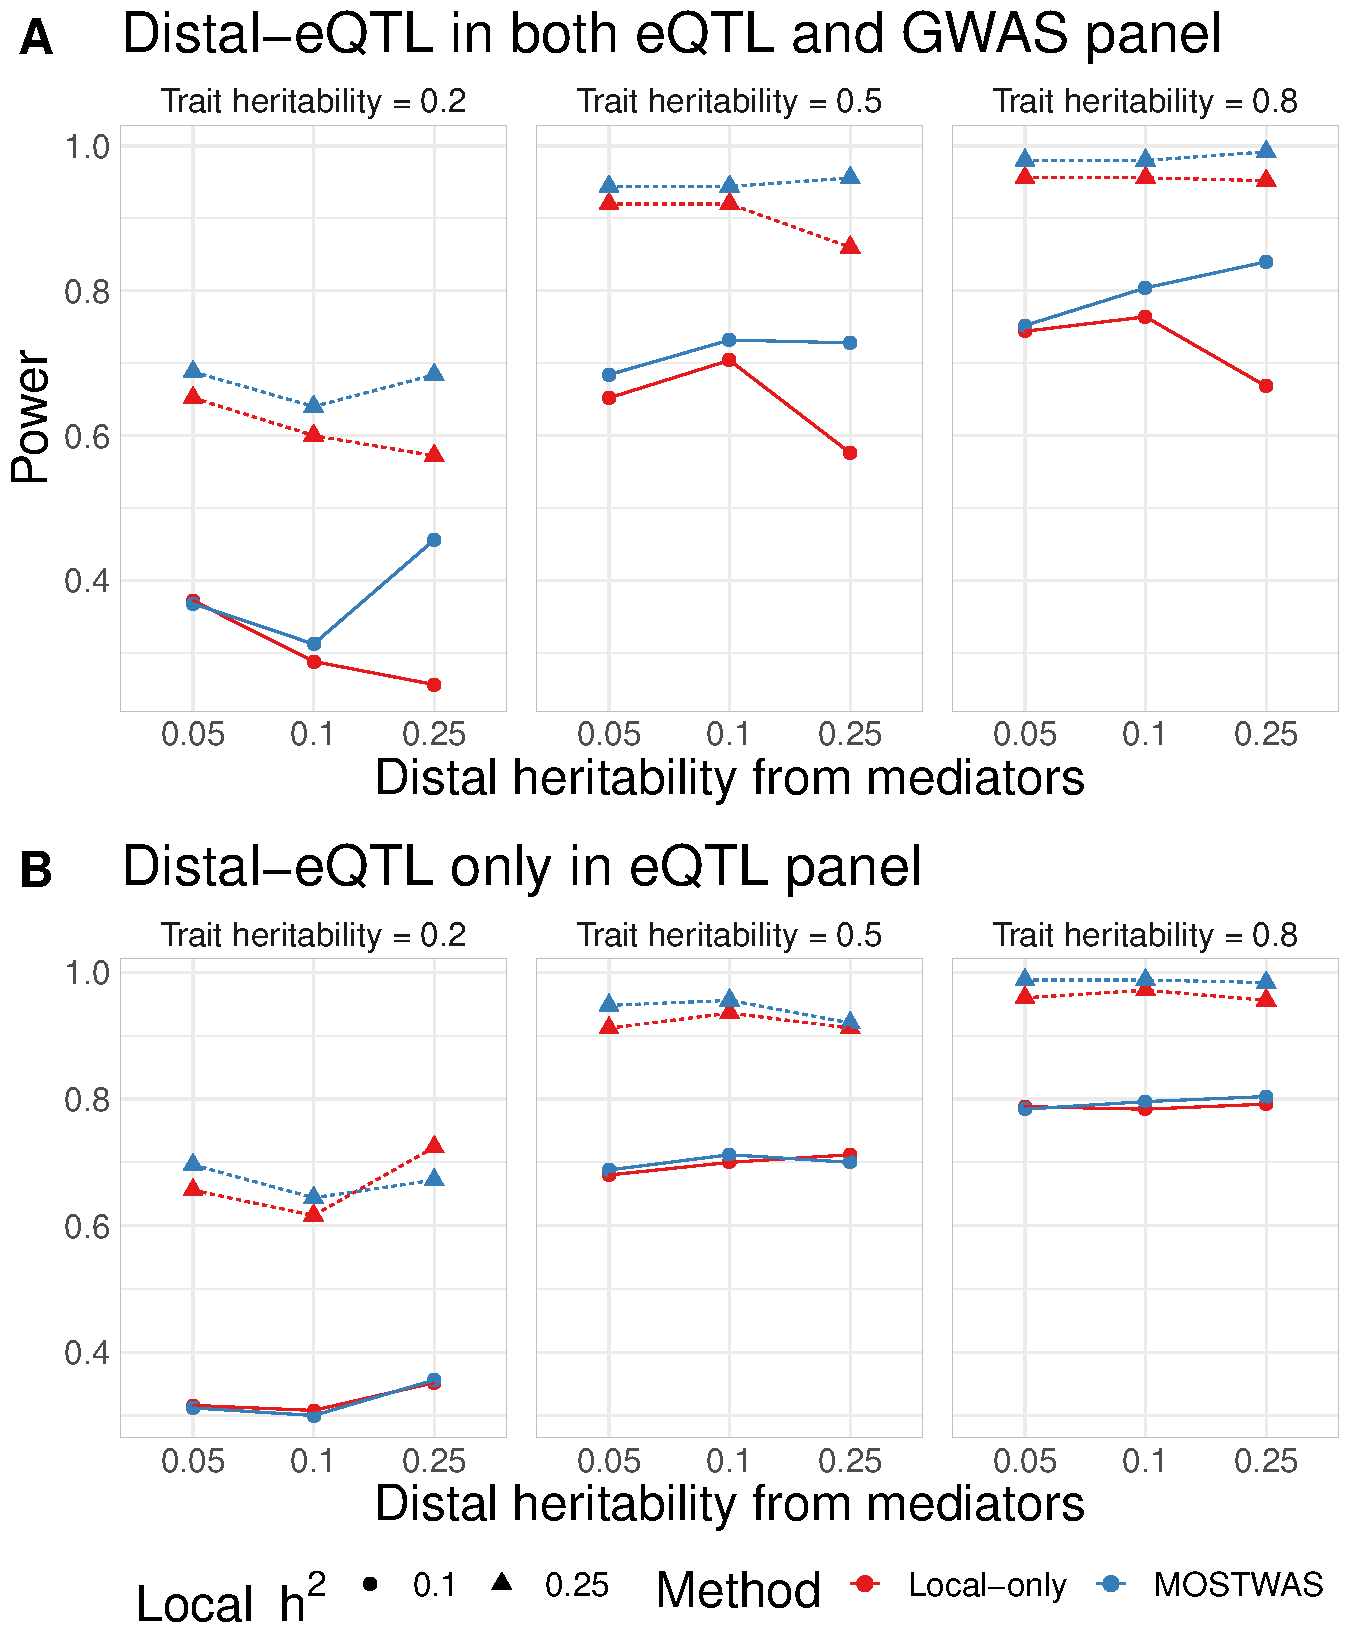
\includegraphics[width = .7\textwidth]{figures/ch4_fig3.pdf}
	\caption{\emph{Comparison of
	TWAS power via simulations
	using MOSTWAS and local-only models.} (A)
	Proportion of gene-trait associations
	at $P < 2.5 \times 10^{-6}$ using local-only (red)
	and the most predictive MOSTWAS (blue) models
	across various local and distal expression heritabilities,
	trait heritability, and causal proportions. (B)
	Proportion of significant gene-trait associations
	across the same simulation parameters with
	no distal effect on the trait in the simulated 
	external GWAS panel.}
	\label{fig:ch4_fig3}
\end{figure}

\subsection{Real data application in breast cancer tumors}

We applied MOSTWAS in the context
of breast tumor multi-omics and
disease outcomes, motivated by recent
GWAS and TWAS into breast cancer-specific survival \cite{Khan2018,Michailidou2013,Michailidou2015,Guo2015,Bhattacharya2020APopulations}. 
Previous breast tumor eQTL studies have
also revealed several signficant
distal-eQTLs in trait-associated
loci, many of which are in regulatory
or epigenetic hotspots
\cite{Bhattacharya2020APopulations,Quiroz-Zarate2017ExpressionTissue},
motivating our application of MOSTWAS
for breast tumor expression modeling.
Using TCGA-BRCA datasets comprising germline SNPs,
tumor mRNA expression, DNA methylation, and miRNA
expression, we trained MeTWAS,
DePMA, and traditional local-only predictive models 
for the mRNA expression of all genes
with germline heritability $h^2 > 0$
at $P < 0.05$.
Estimates of heritability
for genes were considerably larger
when we considered distal variation
using MOSTWAS methods 
(mean heritabilities in \textbf{Supplemental
Table \ref{tbl:ch4_supptab1}}).
We also found that MeTWAS and DePMA
perform better in cross-validation
$R^2$,
with larger numbers of 
models at $R^2 \geq 0.01$
and significant germline heritability
at raw $P < 0.05$
using MOSTWAS methods than
local-only models (\textbf{Figures 
\ref{fig:ch4_fig4}A-C}).
Mean predictive $R^2$
for local-only models was
0.011 (25\% to 75\% inter-quartile
interval (0.0,0.013)), for
MeTWAS models was
0.028 (0.013, 0.032),
and for DePMA models was
0.051 (0.019, 0.068).

In addition to cross-validation,
we used 351 samples in TCGA-BRCA
with only genotype and mRNA expression data
that were not used in model training to
test the portability
of MOSTWAS models in independent
external cohorts. As shown in
\textbf{Figure \ref{fig:ch4_fig5}A and
Supplementary Figure \ref{fig:ch4_suppfig3_5}},
DePMA models obtain the highest
predictive adjusted $R^2$ in
the external cohort (mean 0.016, 25\% to 75\% inter-quartile
interval (0.003, 0.018)), 
with local-only
models (0.013, (0.00,0.013))
outperforming MeTWAS models (0.011,
(0.002, 0.012)),
considering only genes that attained
cross-validation adjusted $R^2 \geq 0.01$
using a given method. Overall,
among genes with cross-validation
adjusted $R^2 \geq 0.01$, 37 out of 280 genes achieved
external predictive $R^2 \geq 0.01$
using local-only models, 89 out of 709 using
MeTWAS, and 787 out of 1,185 using DePMA
(\textbf{Figure \ref{fig:ch4_fig4}A-C}).

Lastly, we conducted association studies
for breast cancer-specific survival
using local-only and the MOSTWAS model with largest
$R^2$ trained
in TCGA-BRCA and summary-level GWAS
data from iCOGs.
Here, we constructed the weighted
burden test, as described above and in Pasaniuc
\etal{} and Gusev \etal{}
\cite{Pasaniuc2014FastEnrichment,Gusev2016}.
We prioritized genes with 
Benjamini-Hochberg \cite{Benjamini1995} adjusted $P < 0.05$
for permutation testing.
Of the 122 genes
that had cross-validation $R^2 \geq 0.01$
in TCGA-BRCA using both local-only
and MOSTWAS models, we found 2 survival
associations with the same loci 
at Benjamini-Hochberg FDR-adjusted 
$0.05$ using both local-only
and MOSTWAS models,
with the strength
of association marginally larger with
the MOSTWAS model in each case (\textbf{Supplemental Figure
\ref{fig:ch4_suppfig2}}).
Furthermore, we find that 116 of these loci
showed larger strengths of association
with survival using the MOSTWAS model
than the local-only model (\textbf{Supplemental Figure
\ref{fig:ch4_suppfig2}}).
QQ-plots for TWAS $Z$-statistics
are provided in \textbf{Supplemental Figure
\ref{fig:ch4_suppfig3}B}
for both local-only and MOSTWAS models.
These results in TCGA-BRCA demonstrated the improved
transcriptomic prediction and power
to detect gene-trait associations using MOSTWAS
over local-only modeling.

\subsubsection{Functional hypothesis
generation with MOSTWAS}

We next conducted TWAS
for breast cancer-specific 
survival using all genes
with significant germline
heritability at $P < 0.05$
with the MOSTWAS model with larger
cross-validation $R^2 > 0.01$.
We identified 21 survival-associated loci
at Benjamini-Hochberg FDR adjusted $P < 0.05$
Of these 21 loci, 11 
persisted when subjected to permutation
testing at a significance threshold of FDR-adjusted $P < 0.05$
(\textbf{Figure \ref{fig:ch4_fig5}C}
and \textbf{Supplemental Table \ref{tbl:ch4_supptab11}}).

An advantage of MOSTWAS is its ability
to aid in functional hypothesis generation
for mechanistic follow-up studies.
The added-last test allows users to
identify genes where trait association
from distal variation is significant above and beyond the
contribution of the local component.
For 8 of the TWAS-associated 11 loci, at
FDR-adjusted $P < 0.05$,
we found significant distal variation added-last
associations (see \textbf{Supplemental Methods}
and \textbf{Supplemental Table \ref{tbl:ch4_supptab11}}), 
suggesting that
distal variation may contribute to the gene-trait
association. All 8 of these loci
showed distal association with
the gene of interest mediated through
a set of four transcription factors 
(\textit{NAA50}, \textit{ATP6V1A}, 
\textit{ROCK2}, \textit{USF3}),
all highly interconnected with the critical MAPK
pathway 
\cite{Dorfel2015TheDisease,Lambertz2015BiologyTreatment,Whitton2018VacuolarCancer,Matsubara2016InhibitorsContext,Chang2018ROCKCells,NiGermlineCarcinoma}. 
These regulatory sites 
serve as an example
of how distal genomic regions 
can be prioritized for
functional follow-up studies to elucidate
the mechanisms underlying the SNP-gene-trait
associations.
These results show the
strength of MOSTWAS to detect and prioritize 
gene-trait
associations that are influenced
by distal variation.

\subsection{Real data application in brain tissue}

We also applied MOSTWAS to transcriptomic data 
on samples of prefrontal cortex,
a tissue that has been used previously
in studying neuropsychiatric traits and disorders
with TWAS \cite{Gusev2018,Raj2018IntegrativeSusceptibility}.
There has been ample evidence in brain tissue, especially the prefrontal
cortex, that non-coding variants
may regulate distal genes \cite{Blauwendraat2016ComprehensiveLobe,Gusev2018,Sey2020AProfiles}; 
in fact, an eQTL analysis
by Sng \etal{} found that approximately
20-40\% of eQTLs in the frontal cortex
can be considered trans-acting \cite{Sng2019Genome-wideDataset}. 
Thus,
the prefrontal cortex in the
context of neuropsychiatric disorders provides a prime
example to assess MOSTWAS.
Using ROS/MAP data on germline SNPs,
tumor mRNA expression, DNA methylation, and miRNA
expression, we trained MeTWAS,
DePMA, and traditional local-only predictive models 
for the mRNA expression of all genes
with germline heritability $h^2 > 0$
at $P < 0.05$. Consistent with results
in TCGA-BRCA, estimates of heritability
for genes were considerably larger
when we considered distal variation
using MOSTWAS methods (\textbf{Supplemental Table \ref{tbl:ch4_supptab1}}).
We also find that MeTWAS and DePMA
perform better in cross-validation
$R^2$ than local-only models (\textbf{Figures 
\ref{fig:ch4_fig4}D-F}).
Mean predictive $R^2$
for local-only models was
0.029 (25\% to 75\% inter-quartile
interval (0.0,0.015)), for
MeTWAS models was
0.079 (0.019, 0.082),
and for DePMA models was
0.045 (0.013, 0.037).

In addition to cross-validation,
we used 87 samples in ROS/MAP
with genotype and mRNA expression data
that were not used in model training to
test the portability
of MOSTWAS models in independent
external cohorts. As shown in
\textbf{Figure \ref{fig:ch4_fig5}A and
Supplementary Figure \ref{fig:ch4_suppfig3_5}},
DePMA models obtain the highest
predictive adjusted $R^2$ in
the external cohort (0.042 (25\% quantile 0.009, 75\% quantile 0.057)), 
with MeTWAS models (0.040 (0.010, 0.054)) also outperforming
local-only
models (0.031 (0.007, 0.039)),
considering only genes that attained
cross-validation adjusted $R^2 \geq 0.01$
using a given method. Overall,
among genes with cross-validation
adjusted $R^2 \geq 0.01$, 187 out of 267 genes achieved
external predictive $R^2 \geq 0.01$
using local-only models, 683 out of 911 using
MeTWAS, and 2,135 out of 2,934 using DePMA
(\textbf{Figure \ref{fig:ch4_fig4}D-F}).

We next conducted association tests
for known Alzheimer's disease risk
loci using local-only and the best MOSTWAS model
(comparing MeTWAS and DePMA cross-validation $R^2$) 
trained
in ROS/MAP and summary-level GWAS
data from IGAP.
From literature, we identified
14 known common and rare loci of late-onset
Alzheimer's disease
\cite{Lambert2013Meta-analysisDisease,Reitz2014GeneticDisease,Sims2017RareDisease,Yuan2017TheDisease},
11 of which had MOSTWAS models
with cross-validation $R^2 \geq 0.01$.
Five of these 11
loci 
(\textit{APOE}, \textit{CLU}, 
\textit{PLCG2}, \textit{SORL1}, 
\textit{ZCWPW1}) showed significant association
at Benjamini-Hochberg FDR-adjusted $P \leq 0.05$
(\textbf{Supplemental Table \ref{tbl:ch4_supptab2}}).
We also compared these 11 associations to
those identified by local-only models
and by latent Dirichlet process regression (DPR)
as implemented in TIGAR \cite{Nagpal2019},
with raw $P$-values of association
shown in \textbf{Figure \ref{fig:ch4_fig5}B}.
MOSTWAS showed stronger associations at 8 of these
loci than both local-only
and DPR models. We followed up on
the 5 significantly associated loci
using the permutation
and added-last tests (see \textbf{Methods} and
\textbf{Supplemental Materials}).
Three of these loci 
(\textit{APOE}, \textit{SORL1}, \textit{ZCWPW1})
showed significant associations, conditional
on large GWAS effect sizes (permutation test 
significant at FDR-adjusted $P < 0.05$)
These three 
loci also showed significant associations with
distal variants, given the association with
local variants, at FDR-adjusted $P < 0.05$ (\textbf{Supplemental 
Table \ref{tbl:ch4_supptab2}}).

We then conducted a transcriptome-wide
association study for risk of major
depressive disorder (MDD) using
summary statistics from the Psychiatric
Genomics Consortium (PGC) genome-wide meta-analysis
that excluded data from the UK Biobank and 
23andMe \cite{Wray2018Genome-wideDepression}.
QQ-plots for TWAS $Z$-statistics
are provided in \textbf{Supplemental Figure
\ref{fig:ch4_suppfig3}B}
for both local-only and MOSTWAS models.
Overall, using all heritable genes with
cross-validation $R^2$ with the best MOSTWAS model
in ROS/MAP, we identified 102 MDD risk-associated loci
with FDR-adjusted $P < 0.05$
 that persisted when subjected to permutation
testing at an FDR-adjusted significance threshold of $P < 0.05$
(colored red in \textbf{Figure \ref{fig:ch4_fig5}D}).
We downloaded genome-wide
association study by proxy (GWAX) summary statistics
from the UK Biobank \cite{Liu2017Case-controlDisease} for replication
analysis of loci identified
using PGC summary statistics. We found that 7
of these 102 loci (labelled
in \textbf{Figure \ref{fig:ch4_fig5}D}) also show an association in UK Biobank
GWAX that is in the same
direction as in PGC.
In comparison,
using local-only models,
we identified 11 genes
with significant association
with MDD risk at FDR-adjusted $P < 0.05$
that persisted permutation testing;
however, none of these loci
showed significant associations
in the UK Biobank GWAX
in the same direction as in PGC.
Summary statistics for MOSTWAS associations
in PGC and UK Biobank are provided 
in \textbf{Supplemental Table \ref{tbl:ch4_supptab3}}.
Local-only results are provided in \textbf{Supplemental
Data}.
It is important to note the UK Biobank dataset is not a GWAS 
dataset as it defines
a case of MDD as any 
subject 
who has the disorder or a first-degree relative 
with MDD, leading to lower power
to detect associations in this
dataset. Nonetheless, we believe that  
strong prediction
of predictive models in independent
cohorts and TWAS results across
two independent cohorts provides
an example of the robustness
of models using MOSTWAS.

\begin{figure}[htbp]
	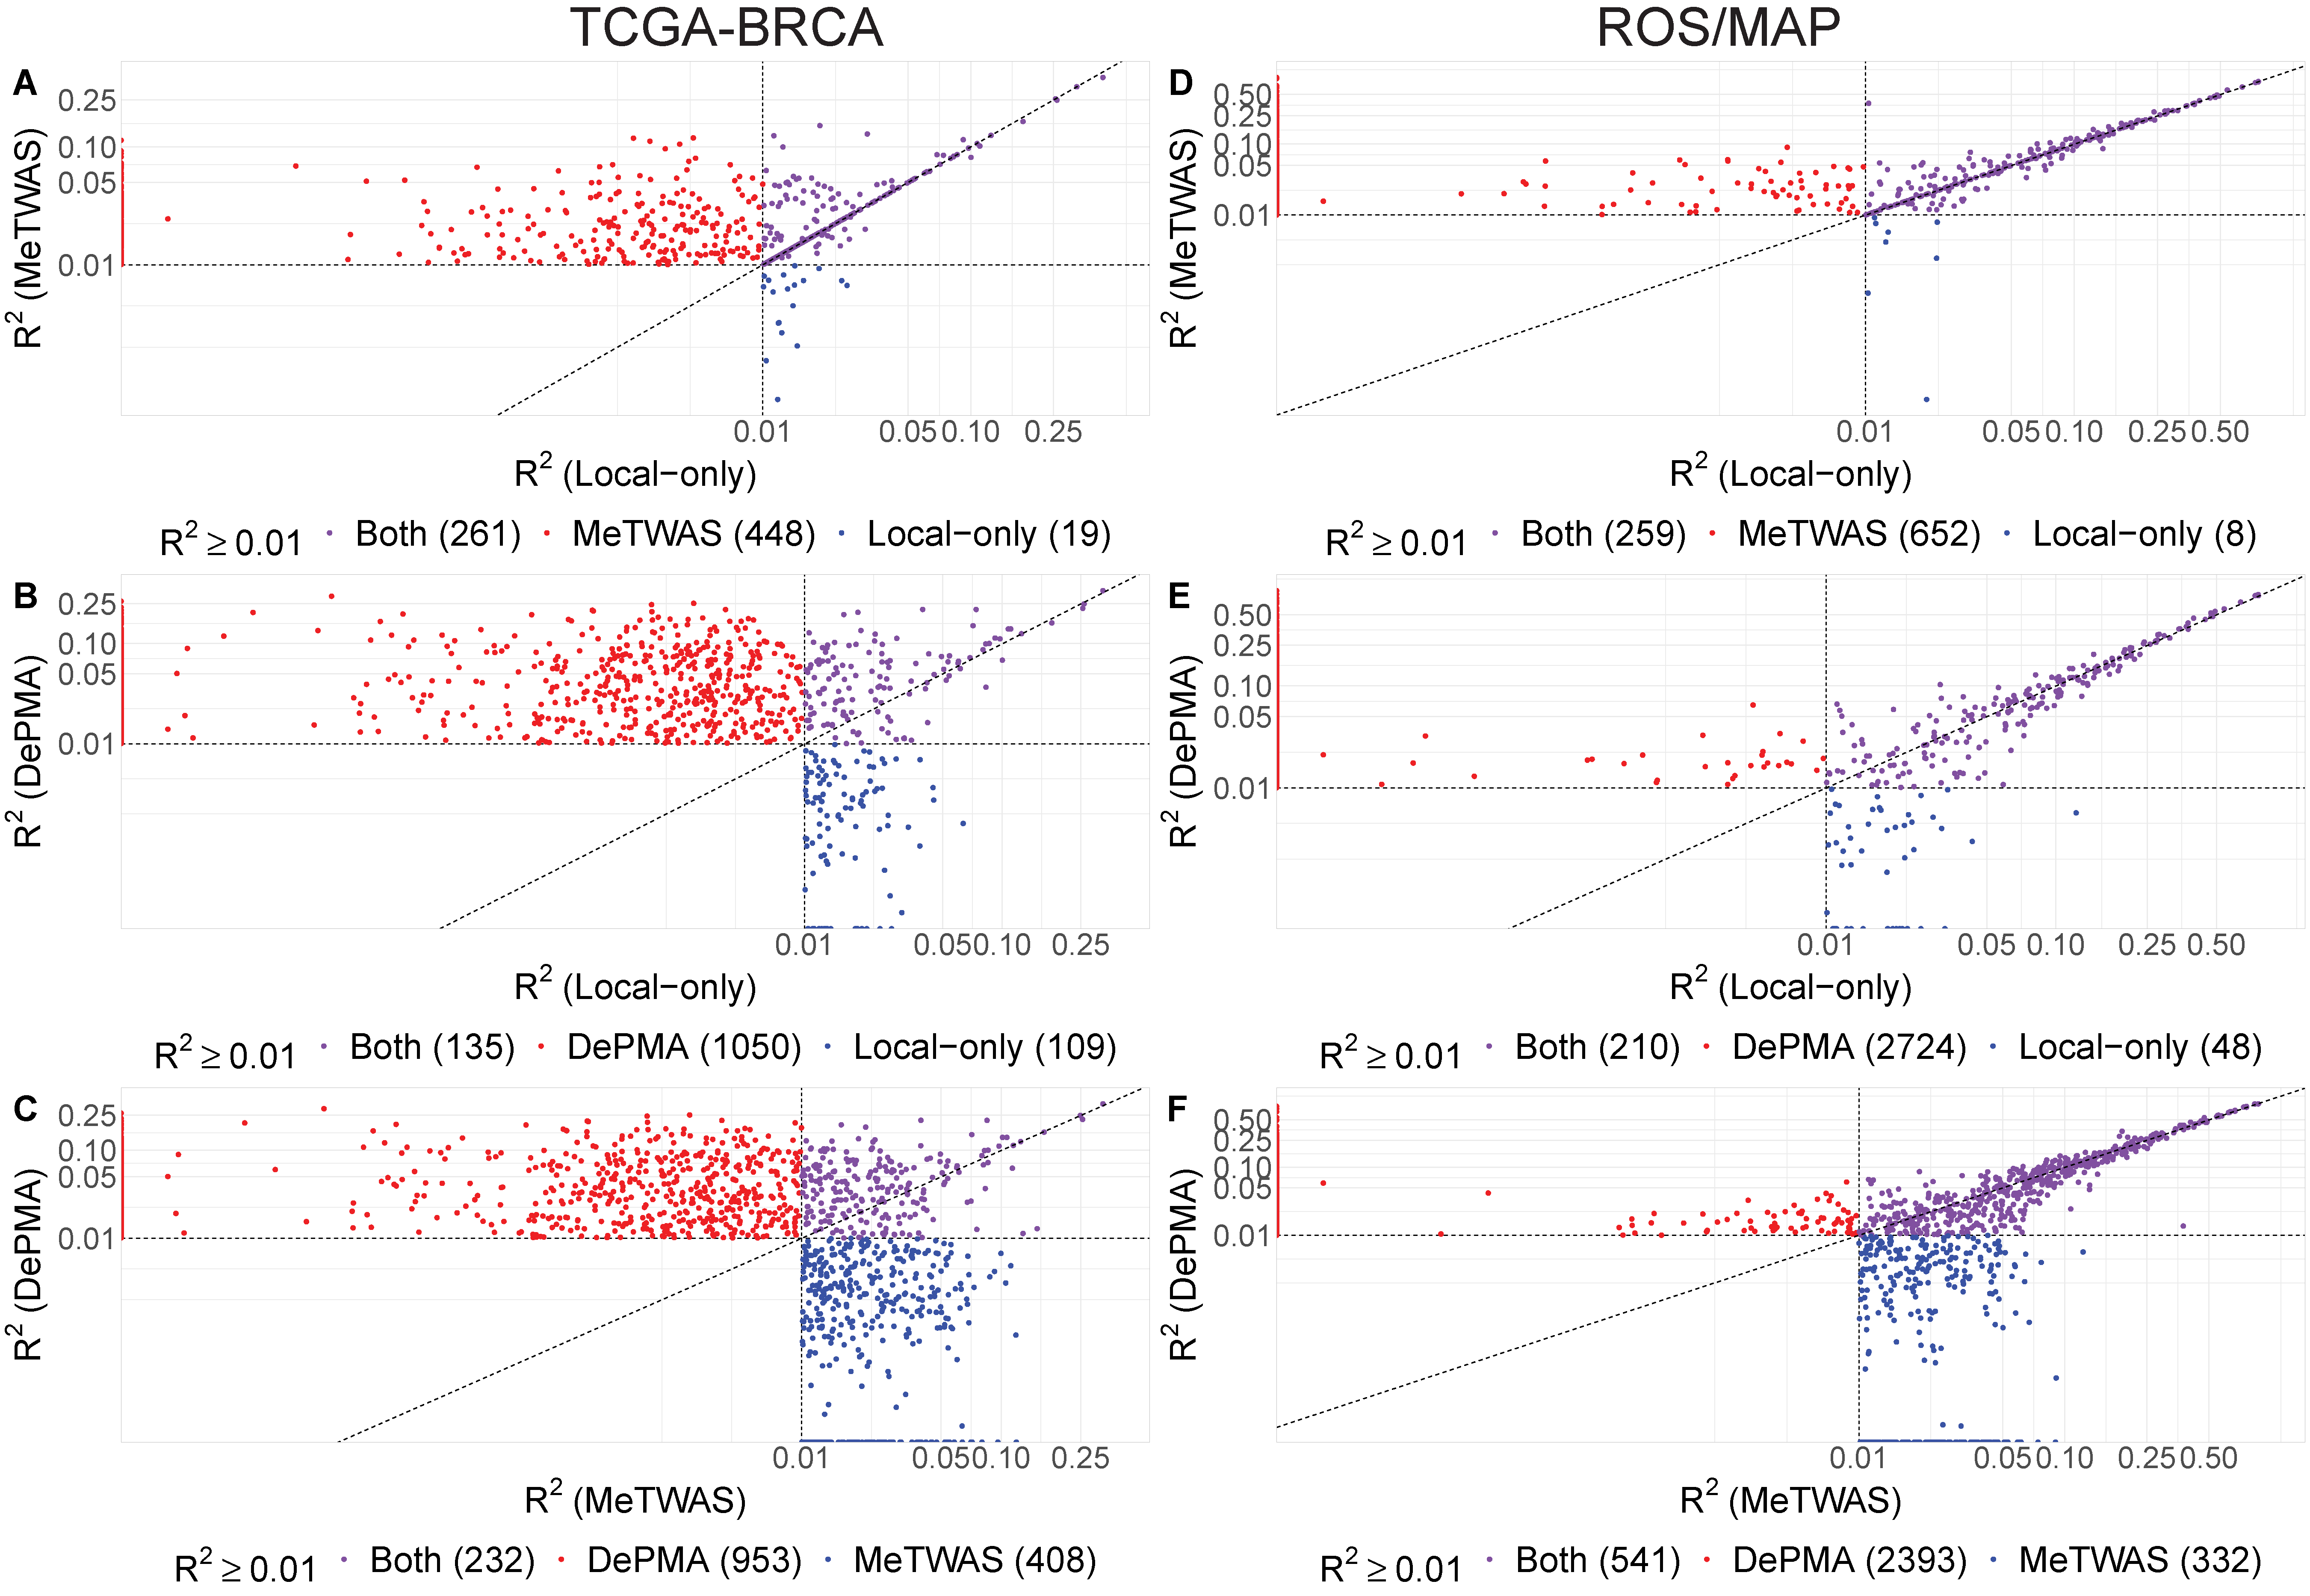
\includegraphics[width = \textwidth]{figures/ch4_fig4.pdf}
	\caption{\emph{Predictive adjusted $R^2$ 
	from cross-validation across
	local-only, MeTWAS, and DePMA
	models.} If a given gene
	does not have $h^2 > 0$
	with $P < 0.05$, we set
	the predictive adjusted $R^2$
	to 0 here for comparison.
	We compare local-only and MeTWAS
	in TCGA-BRCA (A) and ROS/MAP (D),
	local-only and DePMA in TCGA-BRCA (B)
	and ROS/MAP (E), and MeTWAS and DePMA
	in TCGA-BRCA (C) and ROS/MAP (F), all axes indicating the CV
        adjusted $R^2$ for different models.}
	\label{fig:ch4_fig4}
\end{figure}

\begin{figure}[htbp]
	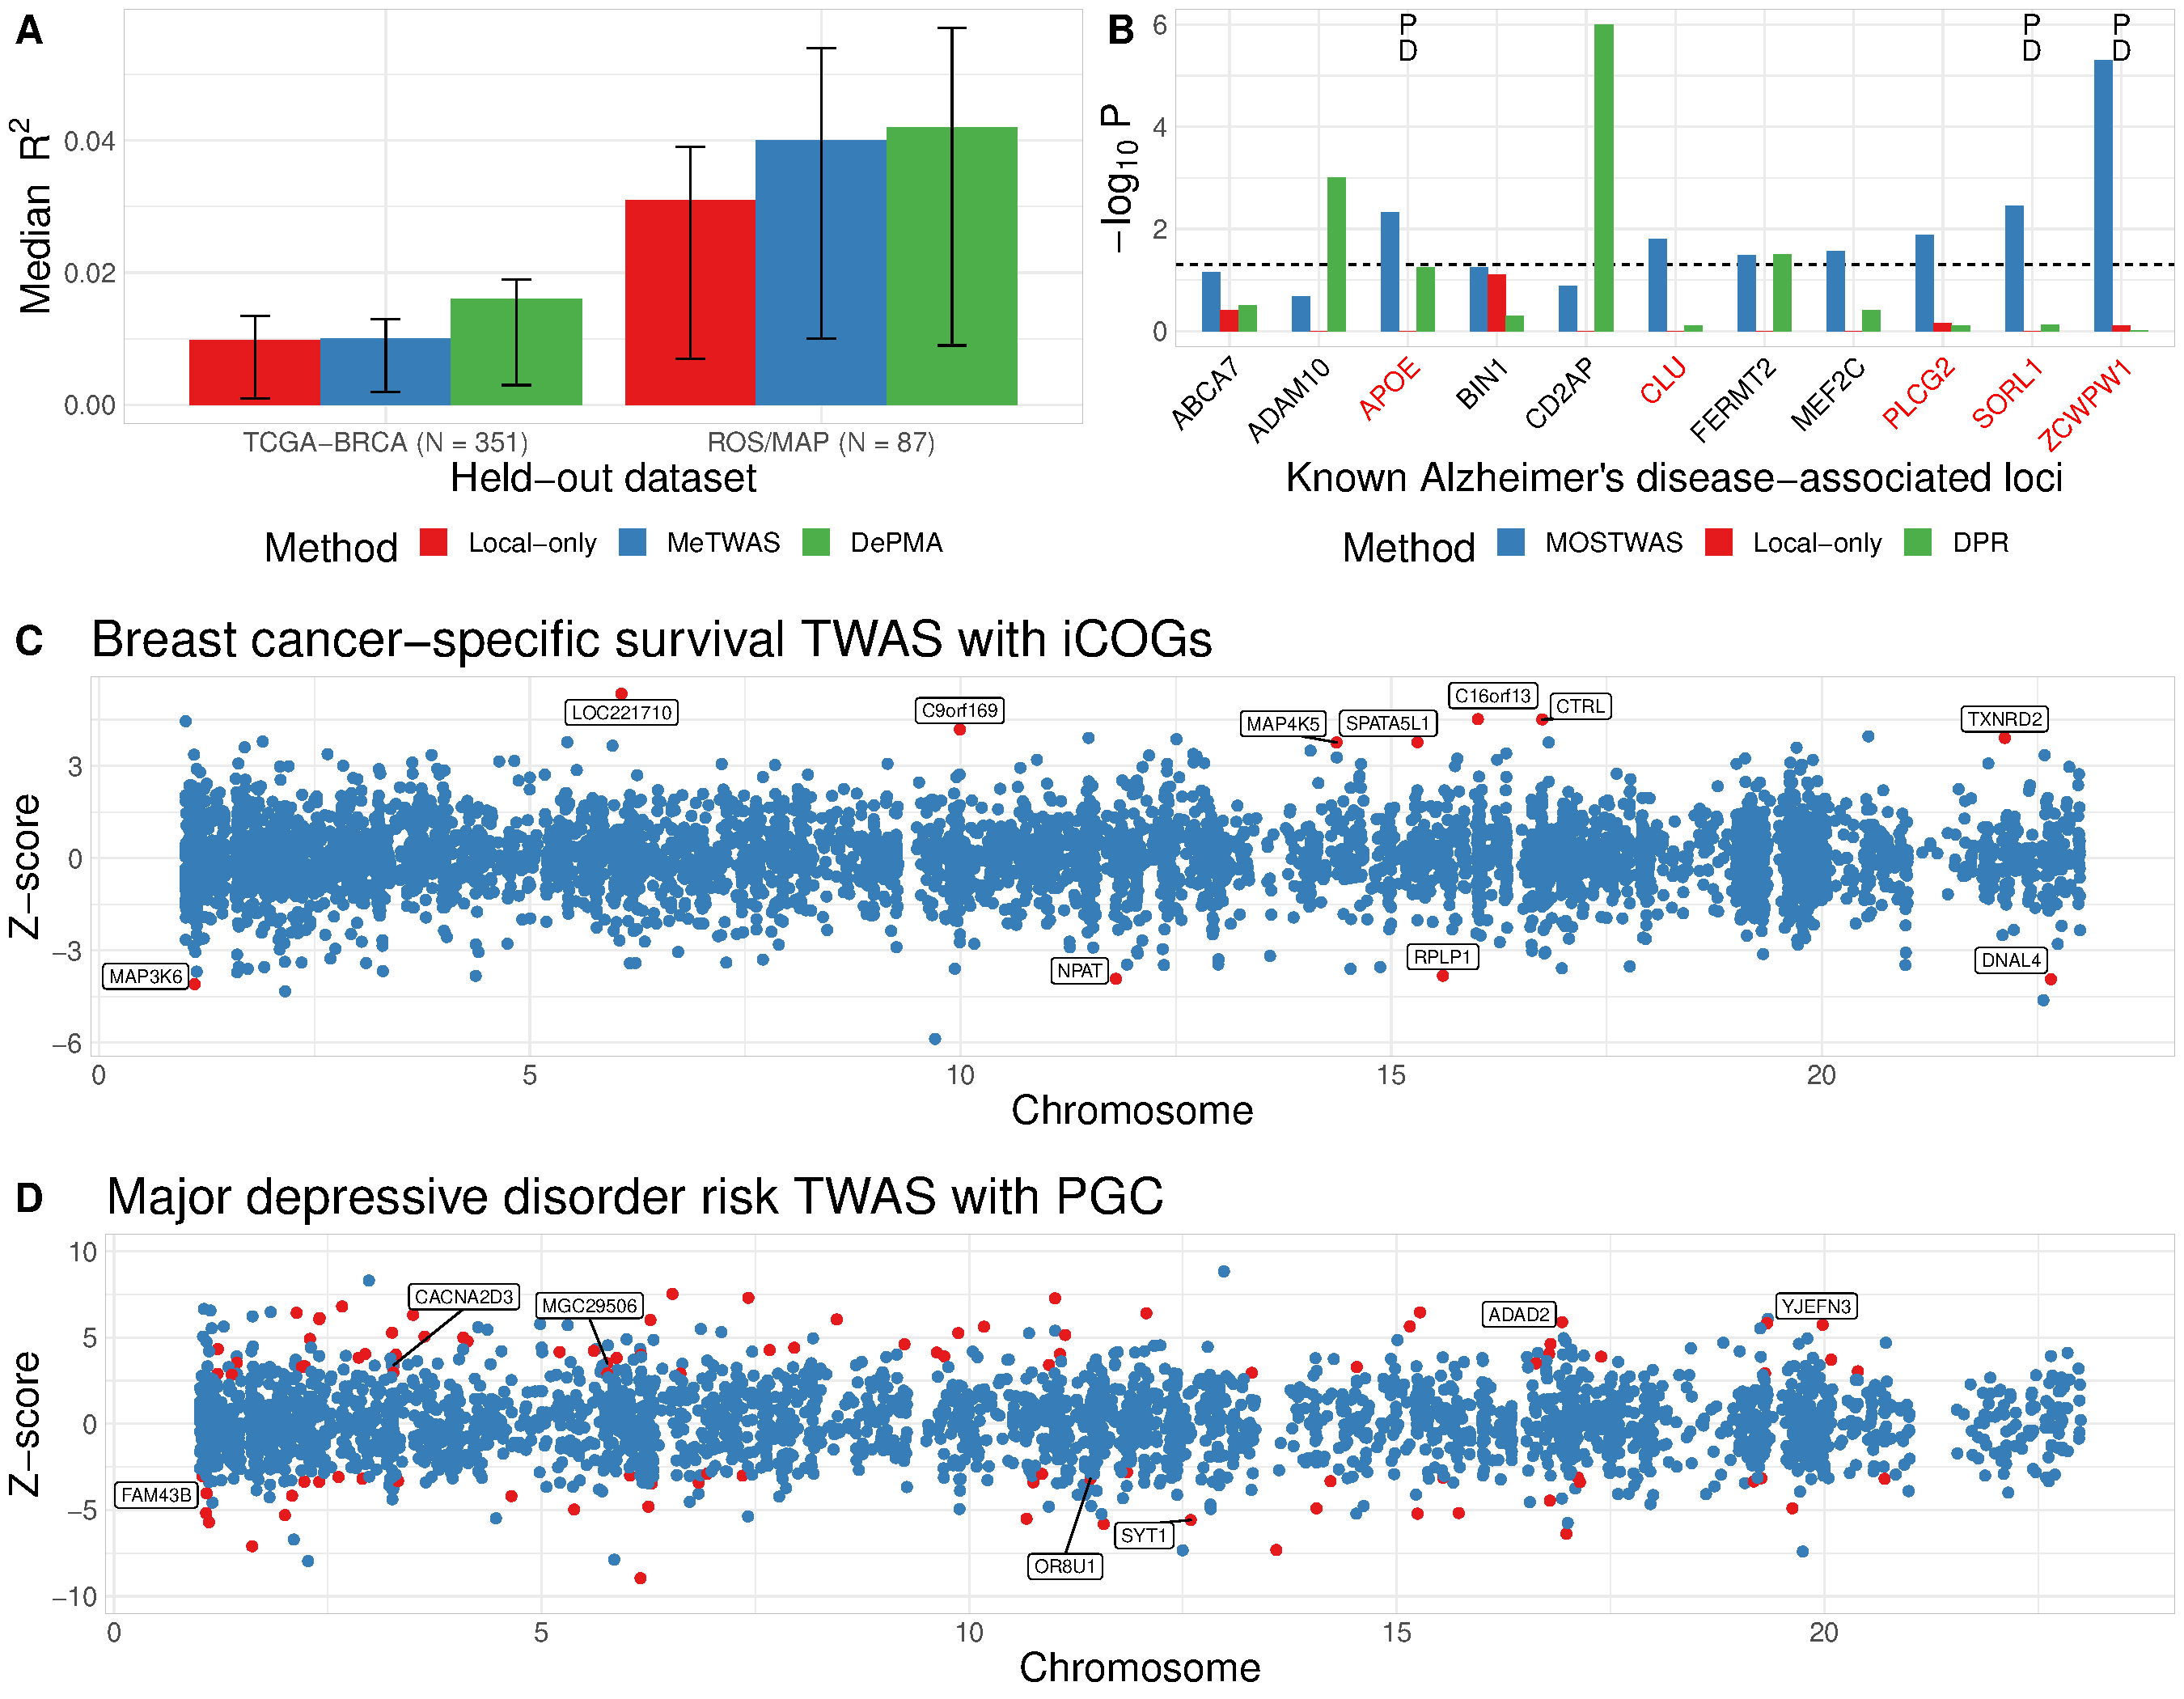
\includegraphics[width = \textwidth]{figures/ch4_fig5.pdf}
	\caption{\emph{External validation of MOSTWAS
	and gene-trait associations
	using MOSTWAS models.} (A) Median predictive
	adjusted $R^2$ in held-out cohorts
	from TCGA-BRCA and ROS/MAP in local-only,
	MeTWAS, and DePMA models that have in-sample significant
	heritability. The interval
	shows the 25\% and 75\% quantiles for external cohort
	predictive $R^2$.
	(B) Associations with 11 known Alzheimer's risk lock,
	as identified in literature, using MOSTWAS, local-only,
	and TIGAR Dirichlet process regression (DPR). (C) TWAS
	associations for breast cancer-specific survival using
	GWAS summary statistics from iCOGs. Loci are colored and
	labelled if the overall association achieves FDR-adjusted 
	$P < 0.05$. Loci
	are labelled with `P' if the permutation test achieves FDR-adjusted $P < 0.05$ and `D' if the added-last
	test achieves FDR-adjusted $P < 0.05$.
	(D) TWAS
	associations for major
	depressive disorder risk using
	GWAS summary statistics from PGC. 
	Loci are colored red if the overall association achieves FDR-adjusted 
	$P < 0.05$ and the permutation test also achieves FDR-adjusted $P < 0.05$.
	We label the 7 loci that
	were independently validated
	with UK Biobank GWAX summary
	statistics at FDR-adjusted
	$P < 0.05$ 
	for both the overall association test
	and permutation test.}
	\label{fig:ch4_fig5}
\end{figure}


We observed that MOSTWAS models generally had 
higher predictive $R^2$ than local-only
models both in training and independent
cohorts. We also found that MOSTWAS
has recapitulated 5 known Alzheimer's
risk loci that were not detected
by local-only modeling (both PrediXcan \cite{Gamazon2015} 
and TIGAR \cite{Nagpal2019}),
3 of which had significant distal associations
using our added-last test.
We also
illustrated that the MOSTWAS detected
MDD-risk loci that were replicable across independent
GWAS and GWAX 
cohorts \cite{Wray2018Genome-wideDepression,Liu2017Case-controlDisease}.

\subsection{Comparison
of computational time}

To assess the difference in computational burden
between local-only, MeTWAS, and
DePMA modelling, we randomly selected a set of 50 genes
that are heritable across all three models
from TCGA-BRCA and computed per-gene
time for fitting using a 24-core, 3.0
GHz processor. We found that 
MeTWAS (mean of 225 seconds
per gene) and DePMA (mean 312 seconds
per gene) took approximately 6-10 times
longer to fit than a traditional local-only model
(mean 36 seconds) 
(\textbf{Supplemental Figure \ref{fig:ch4_suppfig0}}).
Model-fitting here includes heritability
estimation, estimating the SNP-expression
weights, and cross-validation.
We have implemented parallel options
to train an expression model for a single gene 
in MOSTWAS. We also recommend fitting an entire
set of genes from an RNA-seq panel 
via a batch computing
approach \cite{Bischl2015,KoSter2012GenomeEngine}.
Using parallel implementation with 5 cores
and batch computing, we analyzed
15,568 genes from TCGA-BRCA
in approximately 28 hours.

\section{Discussion}
Through a variety of simulations and 
real applications in two settings,
we demonstrate that multi-omic methods 
that prioritize distal variation in TWAS 
have higher predictive performance
and power to detect cell-specific gene-trait 
associations \cite{Brown2013IntegrativeEQTLs,Pierce2018Co-occurringMechanisms,vanderWijst2019Single-cellDisease},
especially when distal variation
contribute substantially to trait heritability.
We proposed two methods (MeTWAS
and DePMA) for
identifying and including distal
genetic variants in gene
expression prediction models.
We have provided implementations of these
methods in the MOSTWAS
(Multi-omic Strategies for Transcriptome-Wide
Association Studies)
R package, available freely
on Github.
MOSTWAS contains functions
to train expression models
with both MeTWAS and DePMA
and outputs models
with 5-fold cross-validation $R^2 \geq 0.01$
and significant germline heritability.
The package also contains functions and documentation
for simulation analyses
\cite{Mancuso2019ProbabilisticStudies},
the weighted burden \cite{Pasaniuc2014FastEnrichment,Gusev2016}
and follow-up permutation \cite{Gusev2016} and distal-SNPs
added-last tests for TWAS
using GWAS summary statistics,
and file-formatting. We also provide
guidelines for parallelization
to lessen computational time.

Not only does MOSTWAS improve
transcriptomic imputation both
in- and out-of-sample, it also provides a test for the 
identification of heritable mediators that affect
eventual transcription of the gene
of interest. These identified mediators
can provide insight into the
underlying mechanisms
for SNP-gene-trait associations
to improve
detection of gene-trait
associations and to prioritize biological units for functional
follow-up studies.
Using MOSTWAS and iCOGs
summary-level GWAS statistics
for breast cancer-specific survival \cite{Guo2015}, we
identified 11 survival-associated loci
that are enriched for p53 binding and
oxidoreductase activity 
pathways \cite{Bao2017P53Context,Zhou2016SystematicState}.
These loci include two genes 
(\textit{MAP3K6} and \textit{MAP4K5}) encoding
mitogen-activated protein kinases, which are 
signalling transduction molecules 
involved in 
the progression of aggressive
breast cancer hormone subtypes
\cite{Ahmad2016ClinicopathologicalCancers}.
TWAS using MOSTWAS models
was able to recapitulate 5 out of 14 known
Alzheimer's disease risk loci
in IGAP GWAS summary statistics
\cite{Lambert2013Meta-analysisDisease},
which were not recoverable
with local-only models.
We showed the utility of 
the distal-SNPs added-last test
to prioritize significant distal SNP-gene-trait
associations
for follow-up mechanistic studies,
which could not be identified 
using traditional local-only TWAS.
In PGC GWAS summary-level data
for major depressive disorder
\cite{Wray2018Genome-wideDepression},
we found 102 risk loci, 7 of which
were replicated in independent
GWAX summary statistics from the UK
Biobank \cite{Liu2017Case-controlDisease}.
Three of these seven loci (\textit{SYT1}, 
\textit{CACNA2D3}, 
\textit{ADAD2})
encode important proteins
involved in synaptic transmission in the brain
and RNA editing. Studies have shown that variation
at these loci may lead to loss
of function at synapses and RNA editing
that lead to psychiatric disorders
\cite{Ryan2006GeneGenes,Baker2015IdentificationCycling,Heyes2015GeneticDisorders,Savva2012TheFamily,Slotkin2013Adenosine-to-inosineDisease}.
All survival- or risk-associated loci identified by MOSTWAS
were not detected using local-only models.

A considerable limitation
of MOSTWAS is the 
increased computational burden
over local-only modelling, especially
in DePMA's permutation-based mediation
analysis for multiple genome-wide mediators.
We believe a Monte-Carlo resampling
method will aid
in scalability by making 
some standard
distributional assumptions
on the effect sizes of
SNPs and mediators in the DePMA
mediation model
\cite{Preacher2012AdvantagesEffects}.
Nevertheless, we believe that MOSTWAS's gain
in predictive performance 
and power to detect gene-trait associations
may outweigh this computational time.
In addition,
RNA-sequencing alignment errors
can lead to false positives in
distal-eQTL detection \cite{Saha2019FalseApproved}, 
and in turn,
bias the mediation modeling.
Cross-mapping estimation, as
described by Saha \etal{} \cite{Saha2019FalseApproved},
can be used to flag potentially falsely
positive distal-QTLs that are detected
as the first step in MeTWAS and DePMA.
Another limitation of MOSTWAS is
the general lack of rich multi-omic
panels, like TCGA-BRCA and ROS/MAP,
that provide a large set of
mediating biomarkers that
may be mechanistically involved
in gene regulation.
However, the two-step regression
framework outlined in MeTWAS
allows for importing
mediator intensity models
trained in other cohorts
to estimate
the germline portion
of total gene expression from
distal variants.

In conclusion,  
MOSTWAS provides a user-friendly
and intuitive tool that extends 
transcriptomic imputation and
association studies to include
distal genetic variants. 
We demonstrated that the methods
in MOSTWAS based on
two-step regression and mediation
analysis generally out-perform
local-only models in
both transcriptomic prediction and TWAS power,
though at the cost of longer computational times.
MOSTWAS enables users to utilize rich reference multi-omic 
datasets for enhanced gene 
mapping to better understand 
the genetic etiology of polygenic traits
and diseases with more direct insight into
functional follow-up studies.

\section{Supplemental Data}

\noindent Document S1: Supplementary Methods,
Supplementary Figures 1--6, Supplementary
Tables 1--4 (supplement.pdf)

\section{Web Resources}

MOSTWAS, \url{https://github.com/bhattacharya-a-bt/MOSTWAS}

TCGA GDC Legacy Archive, \url{https://portal.gdc.cancer.gov/legacy-archive/}

GDAC Firehose Browser, \url{https://gdac.broadinstitute.org/}

ROS/MAP data, \url{https://www.synapse.org/#!Synapse:syn3219045}

IGAP data, \url{http://web.pasteur-lille.fr/en/recherche/u744/igap/igap_download.php}

PGC data, \url{https://www.med.unc.edu/pgc/download-results/mdd/}

UKBB GWAX data, \url{http://gwas-browser.nygenome.org/downloads/gwas-browser/}

\section{Declaration of Interests}

The authors have no competing interests.

\section{Acknowledgements}
We thank Colin Begg, Terry Furey, Michael Gandal, 
Yun Li, Karen Mohlke, Brandon Pierce, Bogdan Pasaniuc,
Hudson Santos, and Jason Stein for
engaging conversation and 
guidance during the research process.

Funding for BCAC and iCOGS
came from: Cancer Research 
UK [grant numbers C1287/A16563,
C1287/A10118, C1287/A10710,
C12292/A11174, C1281/A12014, 
C5047/A8384, C5047/A15007, C5047/A10692,
C8197/A16565], the European Union’s
Horizon 2020 Research and Innovation
Programme (grant numbers 634935 and
633784 for BRIDGES and B-CAST
respectively), the European Community’s
Seventh Framework Programme under grant
agreement n$^\circ$ 223175
[HEALTHF2-2009-223175] (COGS), the
National Institutes of Health [CA128978]
and Post-Cancer GWAS initiative [1U19
CA148537, 1U19 CA148065-01 (DRIVE) and
1U19 CA148112 - the GAME-ON initiative],
the Department of Defence
[W81XWH-10-1-0341], and the Canadian
Institutes of Health Research CIHR) for
the CIHR Team in Familial Risks of Breast
Cancer [grant PSR-SIIRI-701]. All studies
and funders as listed in Michailidou K et
al (2013 and 2015) and in Guo Q et al
(2015) are acknowledged for their
contributions.

We thank the International Genomics of
Alzheimer's Project (IGAP) for providing
summary results data for these analyses.
The investigators within IGAP contributed
to the design and implementation of IGAP
and/or provided data but did not
participate in analysis or writing of
this report. IGAP was made possible by
the generous participation of the control
subjects, the patients, and their
families. The i–Select chips was funded
by the French National Foundation on
Alzheimer's disease and related
disorders. EADI was supported by the
LABEX (laboratory of excellence program
investment for the future) DISTALZ grant,
Inserm, Institut Pasteur de Lille,
Université de Lille 2 and the Lille
University Hospital. GERAD was supported
by the Medical Research Council 
(Grant n$^\circ$)
503480), Alzheimer's Research UK (Grant
n$^\circ$ 503176), the Wellcome Trust
(Grant n$^\circ$ 082604/2/07/Z) and
German Federal Ministry of Education and
Research (BMBF): Competence Network
Dementia (CND) grant n$^\circ$ 01GI0102,
01GI0711, 01GI0420. CHARGE was partly
supported by the NIH/NIA grant R01
AG033193 and the NIA AG081220 and AGES
contract N01–AG–12100, the NHLBI grant
R01 HL105756, the Icelandic Heart
Association, and the Erasmus Medical
Center and Erasmus University. ADGC was
supported by the NIH/NIA grants: U01
AG032984, U24 AG021886, U01 AG016976,
and the Alzheimer's Association grant
ADGC–10–196728.

We also thank the
Psychiatric Genomics Consortium
for their publicly
available GWAS summary statistics
(\url{https://www.med.unc.edu/pgc/})
and the
Pickrell Lab at the
New York Genome Center for
their GWAS browser
and GWAX summary statistics
(\url{http://gwas-browser.nygenome.org/downloads/gwas-browser/}).
 


\section{Accession Numbers}

Birdseed genotype files of 914 subject were downloaded
from the Genome Data Commons (GDC)
legacy (GRCh37/hg19) archive
(\url{https://portal.gdc.cancer.gov/legacy-archive/}).
Processed mRNA/miRNA expression
and CpG methylation data was
accessed from the Firehose repository
from the Broad Institute via FireBrowse
(\url{https://gdac.broadinstitute.org/}) \cite{Weinstein2013TheProject}.
ROS/MAP multiomics data (genotype,
mRNA and miRNA expression, CpG methylation)
was accessed through 
the AMP-AD Knowledge
Portal on Synapse (Synapse ID: syn3219045) \cite{DeJager2018DataResearch}.

\bibliography{library}

\end{document}
